\documentclass[12pt]{article} % Document type
\usepackage[utf8]{inputenc}

\usepackage{amsmath, amssymb, amsthm, amssymb}
\usepackage{mathdots}
\usepackage[pdftex]{graphicx}
\usepackage{fancyhdr}
\usepackage[margin=1in]{geometry}
\usepackage{multicol}
\usepackage{bm}
\usepackage{listings}
\PassOptionsToPackage{usenames,dvipsnames}{color}  %% Allow color names
\usepackage{pdfpages}
\usepackage{algpseudocode}
\usepackage{tikz}
\usepackage{enumitem}
\usepackage[T1]{fontenc}
\usepackage{inconsolata}
\usepackage{framed}
\usepackage{wasysym}
\usepackage[thinlines]{easytable}
\usepackage{wrapfig}
\usepackage{hyperref}
\usepackage{mathrsfs}
\usepackage{tabularx} % also loads 'array' package
\usepackage{diagbox}

\title{Quantitative and Local Central Limit Theorems}
\author{}
\date{}

\lhead{}
\chead{}
\rhead{}
\lfoot{}
\cfoot{}
\rfoot{\thepage}

\definecolor{shadecolor}{gray}{0.9}

%%%%%%%%%%%%%%%%%%%%
%%%%%%%%%%%%%%%%%%%%
%
% Custom spacing commands

\newcommand{\sss}{\vspace{2 mm}\noindent}
\newcommand{\lss}{\vspace{5 mm}\noindent}
\newcommand{\lls}{\vspace{7 mm}\noindent}
\newcommand{\ds}{\displaystyle}
\newcommand{\HR}{\vspace{5pt}\hrule height 1pt \vspace{5pt}}
%%%%%%%%%%%%%%%%%%%%
%%%%%%%%%%%%%%%%%%%%
%
% Shortcuts for commonly used symbols

\newcommand{\f}[2]{\frac{#1}{#2}}
\newcommand{\p}[1]{\left(#1\right)}
\newcommand{\s}[1]{\left[#1\right]}
\newcommand{\abs}[1]{\left\lvert#1\right\rvert}

\newcommand{\R}{\mathbb{R}}
\newcommand{\Var}{\mathrm{Var}}

\renewcommand{\P}{\mathbb{P}}
\newcommand{\ap}{\mathcal{A}}
\newcommand{\E}{\mathbb{E}}
\newcommand{\F}{\mathbb{F}}
\newcommand{\ca}{\mathcal}
\newcommand{\fr}{\mathfrak}
\newcommand{\eu}{\EuScript}
\newcommand{\scr}{\mathscr}
\newcommand{\bbn}{\mathbb{N}}
\newcommand{\bbr}{\mathbb{R}}
\newcommand{\bbq}{\mathbb{Q}}
\newcommand{\bbc}{\mathbb{C}}
\newcommand{\Z}{\mathbb{Z}}
\newcommand{\bbp}{\mathbb{P}}
\newcommand{\bfa}{\mathbf{a}}
\newcommand{\bfb}{\mathbf{b}}
\newcommand{\bfc}{\mathbf{c}}
\newcommand{\bfu}{\mathbf{u}}
\newcommand{\bfv}{\mathbf{v}}
\newcommand{\bfx}{\mathbf{x}}
\newcommand{\ring}{\ca O}

\newcommand{\inv}{^{-1}}
\newcommand{\into}{\hookrightarrow}
\newcommand{\onto}{\twoheadrightarrow}
\newcommand{\isom}{\overset{\sim}{\to}}
\renewcommand{\iff}{\Leftrightarrow}
\renewcommand{\implies}{\Rightarrow}
\renewcommand{\impliedby}{\Leftarrow}
\newcommand{\contradiction}{\Rightarrow\Leftarrow}

\newcommand{\norm}[1]{\left\lVert#1\right\rVert}
\renewcommand{\d}{\mathrm{d}}
\newcommand{\eps}{\varepsilon}

%%%%%%%%%%%%%%%%%%%%
%%%%%%%%%%%%%%%%%%%%

%%%%%%%%%%%%%%%%%%%
%%%%%%%%%%%%%%%%%%%
%
% Environment styles

\newtheorem{thm}{Theorem}[section]
\newtheorem{prop}[thm]{Proposition}
\newtheorem{cor}[thm]{Corollary}
\newtheorem{question}[thm]{Question}
\newtheorem{hypothesis}[thm]{Hypothesis}
\newtheorem{lem}[thm]{Lemma}
\newtheorem*{prop*}{Proposition}
\newtheorem*{cor*}{Corollary}
\newtheorem*{lem*}{Lemma}
\newtheorem*{thm*}{Theorem}

\theoremstyle{definition}
\newtheorem{conj}[thm]{Conjecture}
\newtheorem{defn}[thm]{Definition}
\newtheorem{claim}[thm]{Claim}
\newtheorem{example}[thm]{Example}
\newtheorem*{conj*}{Conjecture}
\newtheorem*{rd}{Read from the text}
\newenvironment{answer}{\noindent\textsc{Answer:}}{\hfill $\square$}

\theoremstyle{remark}
\newtheorem*{defn*}{Definition}
\newtheorem{remark}[thm]{Remark}
\newtheorem*{remark*}{Remark}
\newtheorem{notation}[thm]{Notation}

% End of top matter
%
%%%%%%%%%%%%%%%%%%%
%%%%%%%%%%%%%%%%%%%

\begin{document}

\maketitle

%%%%%%%%%%%%%%%%%%%%%%%%%%%%%%%%%%%%%%%
\begin{abstract}
We prove a quantitative local limit theorem for the number of descents in a random permutation. We conjecture that there is no local limit theorem for the number of length 3 arithmetic progressions in a random subset of $\Z/n\Z$, but a proof of this remains elusive. A promising avenue of proof is to condition on the size of the subset and show that the resulting distributions are too far apart for different sizes. This has proven difficult because the distances between these conditioned distributions are extremely close to their standard deviations.
\end{abstract}

\section{Introduction}

Let $\{X_n\}$ be a sequence of discrete random variables taking integer values with mean $\mu_n$ and standard deviation $\sigma_n$. For example, $X_n$ could be the number of heads that occur in $n$ coinflips. The central question is of convergence of the $X_n$. In the example of coinflips, the $X_n$ themselves do not converge in any meaningful way, since $\mu_n$ is increasing in $n$, so we consider convergence of $Y_n = \f{X_n - \mu_n}{\sigma_n}$ to the standard normal distribution $Z$ instead.

One notion of convergence of a sequence of random variables is convergence in distribution \cite{Chatterjee07}. This concerns pointwise convergence of cumulative distribution functions. We write that $\{Y_n\}$ converges in distribution to $Z$, or $Y_n \xrightarrow{d} Z$, if
\[ \abs{\P(Y_n \leq t) - \P(Z \leq t)} \to 0 \]
for each $t \in \R$. If this condition holds, the sequence $\{X_n\}$ satisfies a \textbf{central limit theorem}. The example of coinflips satisfies a central limit theorem. But what if we wanted to know, for instance, the probability of getting exactly half heads, that is, $\P(X_n = n/2)$ (for even $n$)? The central limit theorem only tells us the probability of having at most half heads, that is, $\P(X_n < \f{n}{2}) = \P(Y_n < 0) \to \P(Z < 0) = \f{1}{2}$. We could try to extract a pointwise probability from the central limit theorem by observing
\begin{align*}
	\P(X_n = k)
	&= \P(k - \f{1}{2} < X_n < k + \f{1}{2}) \\
	&= \P((k - \f{1}{2} - \mu_n)/\sigma_n < Y_n < (k + \f{1}{2} - \mu_n)/\sigma_n) \\
	&\to \P((k - \f{1}{2} - \mu_n)/\sigma_n < Z < (k + \f{1}{2} - \mu_n)/\sigma_n).
\end{align*}
% TODO: ^ this is useless, also keep things normalized more
But this is not very helpful, since each quantity simply goes to $0$ as $n$ gets large and there is no bound on the rate of convergence. Another way to phrase it is that
\[ \abs{\P(X_n = k) - \f{1}{\sqrt{2\pi}\sigma_n} e^{-\p{\f{k - \mu_n}{\sigma_n}}^2}} \to 0, \]
but this is trivial since both terms go to $0$. To find an error bound that makes the convergence meaningful, observe that a normal distribution with standard deviation $\sigma$ has height $\Theta(\f{1}{\sigma})$. Therefore, we want
\[ \abs{\P(X_n = k) - \f{1}{\sqrt{2\pi}\sigma_n} e^{-\p{\f{k - \mu_n}{\sigma_n}}^2}} = o\p{\f{1}{\sigma_n}} \]
uniformly in $k$. If this condition holds, the sequence $\{X_n\}$ satisfies a \textbf{local limit theorem}. The existence of local limit theorems is our main area of interest.

\subsection{Descents}

One variable of interest to us is the number of descents in a random permutation. A permutation $\pi$ has a descent at index $i$ if $\pi(i) > \pi(i+1)$. The number of descents in $\pi$, denoted $D(\pi)$, is the number of such indices $i$. We define the indicator random variable for the $i$th descent
\[ X_i = \begin{cases} 1 & \pi(i) > \pi(i+1) \\ 0 & \text{else} \end{cases}, \]
so the number of descents can be written
\[ D_n = \sum_{i=1}^{n-1} X_i. \]
To sample random permutations, uniformly and independently pick random integers $1 \leq a_i \leq n - i + 1$ for each $1 \leq i \leq n$. The $a_i$ correspond to permutations like so: let $S = \{1, \ldots, n\}$, and for each $i$, in order from $1$ to $n$, define $\pi(i)$ to be the $i$th remaining element of $S$, and remove $\pi(i)$ from $S$. Under this correspondence, $\pi(i) > \pi(i+1)$ if and only if $a_i > a_{i+1}$. Therefore, $X_i$ can be equivalently defined by
\[ X_i = \begin{cases} 1 & a_i > a_{i+1} \\ 0 & \text{else} \end{cases}. \]
	With this method of sampling, we can compute some basic facts about $D$. At each index $i$, there is either a descent or an ascent ($\pi(i) < \pi(i+1)$) and these both occur with equal probability, so $\E[X_i] = \f{1}{2}$. Therefore, $\E[D] = \f{n-1}{2}$. With similar reasoning as in computing the expectation of $X_i$, we get $\E[X_i X_{i+1}] = \f{1}{3!} = \f{1}{6}$. Also, it is important to note that $X_i$ is independent of all other $X_j$ except for $X_{i-1}$ and $X_{i+1}$. Now we compute
\begin{align*}
	\Var(D)
	&= \E[D^2] - \E[D]^2 \\
	&= \E\s{\sum_{i=1}^{n-1} \sum_{j=1}^{n-1} X_i X_j} - \p{\f{n-1}{2}}^2 \\
	&= \sum_{i=1}^{n-1} \E[X_i^2] + \sum_{\abs{i-j} = 1} \E[X_i X_j] + \sum_{\abs{i-j} > 1} \E[X_i X_j] - \f{(n-1)^2}{4} \\
	&= \f{n-1}{2} + \f{2(n-2)}{6} + \f{(n-1)^2 - (n-1) - 2(n-2)}{4} - \f{(n-1)^2}{4} \\
	&= \f{n+1}{12}.
\end{align*}

\subsection{Arithmetic Progressions}

The other random variable of interest is the number of length 3 arithmetic progressions (APs) in a random subset of $\Z/n\Z$. We require $n$ odd and $n > 3$ to avoid issues of divisibility. For $1 \leq i \leq n$, let $x_i$ be the indicator random variable for $i \in S \subseteq \Z/n\Z$. The $x_i$ are independent and each has expectation $\f{1}{2}$. We define the number of arithmetic progressions in $S$ as
\[ A_n = \f{1}{2} \sum_{i=1}^{n} \sum_{j=1}^{n-1} x_i x_{i+j} x_{i+2j}. \]
This definition does not consider triples that contain the same element twice to be an arithmetic progression, and the factor of $\f{1}{2}$ causes multiple triples with the same elements to be considered the same progression. The mean of $A_n$ is $\E[A_n] = \f{1}{8}\binom{n}{2}$. The variance of $A_n$ is computed in section 4.


\section{Background}

\subsection{Number of Triangles in a Random Graph}
Previous papers have studied the distribution of the number of triangles $T_n$ in a random graph $G_{n,p}$, which is the undirected graph on $n$ vertices where each of the $n\choose2$ edges have probability $p$ of appearing in the graph. Let $R_n = \frac{T_n-\mu}{\sigma}$ be the normalized $T_n$. The standard normal probability density function $\mathcal{N}(x) = \frac{1}{\sqrt{2\pi}}e^{-x^2/2}.$ Gilmer and Kopparty (ADD CITATION) establish the existence of an LLT for $T_n$. In particular, they show that the distribution of $T_n$ is pointwise approximated by a discrete Gaussian distribution. 
\begin{thm}[Gilmer, Kopparty, 2014]
If $L = \{\frac{k-\mu_n}{\sigma_n}: k \in \Z \} $, as $n \rightarrow \infty$, \[\sup_{x\in L} \abs{\sigma_n P(R_n = x) - \mathcal{N}(x)} \rightarrow 0. \]
\end{thm}

We note that this is a qualitative result, where the error = $o(n^{-2}) = o(\frac{1}{\sigma})$. Berkowitz (ADD CITATION) expanded on their work and established a quantitative bound on the distance between the distribution of $T_n$ and the Gaussian distribution. In particular, he shows the following result:

\begin{thm}[Berkowitz, 2016]
For all $k \in \Z$, \[ P(T_n = k) = \f{1}{\sqrt{2\pi}\sigma_n} \mathrm{exp}\p{-((k-\mu_n)/\sigma_n)^2/2} + o(n^{-2.5+\epsilon}). \]
\end{thm}

\subsubsection{Methods used to establish an LLT for $T_n$}
Here we summarize the methods used by Gilmer and Kopparty (ADD CITATION) in proving that an LLT exists for $T_n$.
With some calculations, we have the mean $\E[T_n] = \mu_n = p^3{n\choose3}$ and the variance $\sigma^2 = \Theta(n^4).$ 
A crucial formula for the proof is the following:
\begin{prop}[Fourier Inversion Formula]
If $Y$ is a random variable with support in the discrete lattice $L = \frac{1}{b}(\Z - a)$ for $a,b \in \bbr$, and $\phi(t) = \E[e^{itY}]$ is the characteristic function of $Y$, then $\forall \ y \in L$, 
\[ P(Y = y) = \frac{1}{2\pi b} \int_{-\pi b}^{\pi b} e^{-ity}\phi(t)\ dt.
\]
\end{prop}

If we let $\phi_n(t) = \E[e^{itR_n}]$, then 
$\sigma_n P(R_n = x) = \frac{1}{2\pi} \int_{-\pi\sigma}^{\pi\sigma} e^{-itx}\phi(t)\ dt.$
By the standard Fourier inversion formula,
$\mathcal{N}(x) = \frac{1}{2\pi} \int_{-\infty}^{\infty} e^{-itx}e^{x^2/2}\ dt.$ Thus, 
\[ \abs{\sigma_n P(R_n = x)} \leq \int_{-\pi\sigma_n}^{\pi\sigma_n} \abs{\phi_n(t) - e^{-t^2/2}} dt + 2 \int_{\pi\sigma_n}^{\infty} e^{-t^2/2}\ dt
\]
Thus, since the second term goes to 0 as n goes to infinity, we just have to show \[\int_{-\pi\sigma_n}^{\pi\sigma_n} \abs{\phi_n(t) - e^{-t^2/2}} dt = o(1)\].

For any constant $A$, we can write
	\[
		\int_{-\pi \sigma}^{\pi \sigma} \abs{\phi_n(t) - e^{-t^2/2}} \d t
		\leq \int_{-A}^{A} \abs{\phi_n(t) - e^{-t^2/2}} \d t
		+ \int_{A \leq \abs{t} \leq \pi \sigma} (\abs{\phi_n(t)} + |e^{-t^2/2}|)
\]

Hence, we have reduced the problem of proving an LLT to one of sufficiently bounding the characteristic function $\abs{\phi_n(t)}$. 
The overall strategy used to bound the $\abs{\phi_n(t)}$ involves finding an event that occurs with high probability and allows $R_n$ to be written as the sum of $n$ i.i.d. random variables $X_i$ after conditioning on the event. Let $F$ be all the edges except for those in a perfect matching $M$, and let $X_F$ be the indicator vector for edges in $F$ that appear in $G$. For any edge $e = \{u,v\}$ in $M$, let $C_e$ be the number of paths from $u$ to $v$ of length 2 that appear in $G$. Now $C_e$ and $C$, the number of triangles with edges only in $F$, are both constants conditioned on $X_F$. Then using a few lemmas (see G-K for details), we can conclude 
\[ \abs{\E[e^{itR_n} | X_F]} = \abs{\E[e^{it(\sum_{e\in M} C_e X_e)/\sigma_n}]} \approx e^{-\Theta(t^2/n)}.
\] The remaining elements and details of the proof are omitted here.  

Using the $p$-biased Fourier basis, Berkowitz shows $\int_{-\pi\sigma_n}^{\pi\sigma_n} \abs{\phi_n(t) - e^{-t^2/2}} dt$ = O($n^{-1/2+\epsilon}$). In section 4 below, we set up and apply this tool for 3-term arithmetic progressions. 


\section{Descents in a Permutation}

Let $\pi \in S_n$ be a permutation. Define $D(\pi) = \abs{\{1 \leq i < n \mid \pi(i + 1) < \pi(i)\}}$ to be the number of descents in $\pi$. Viewing $D_n$ as a random variable on uniformly distributed permutations, a central limit theorem is known and we establish a local limit theorem.

	As another way of viewing a permutation $\pi$, consider a sequence $a_1, \ldots, a_n$ with $1 \leq a_i \leq n - i + 1$. To get a permutation $\pi$ from such a sequence, start with $S = \{1, \ldots, n\}$. For $i = 1, \ldots, n$, let $b_i$ be the $a_i$th remaining element of $S$, let $\pi(i) = b_i$, and remove $b_i$ from $S$. Then $\pi(i + i) < \pi(i)$ if and only if $a_{i+1} < a_i$, so the problem of counting descents in $\pi$ is equivalent to the problem of counting descents in $\{a_i\}$. This is nice since the $a_i$ are distributed independently.

	Now, define the random variable $X_i$ for $1 \leq i < n$ as the indicator for the $i$th potential descent, that is, $1$ if $a_{i+1} < a_i$ and $0$ otherwise. We can write $D_n = X_1 + \ldots + X_n$. Since $X_i$ depends only on $a_i$ and $a_{i+1}$, $X_i$ is independent of all other $X_j$ except for $X_{i-1}$ and $X_{i+1}$. We calculate
	\begin{align*}
		\P(X_i = 1 \mid X_{i-1} = 1, X_{i+1} = 1) &= 1/6 \\
		\P(X_i = 1 \mid X_{i-1} = 1, X_{i+1} = 0) &= 1/2 \\
		\P(X_i = 1 \mid X_{i-1} = 0, X_{i+1} = 1) &= 1/2 \\
		\P(X_i = 1 \mid X_{i-1} = 0, X_{i+1} = 0) &= 5/6.
	\end{align*}
	To bound the characteristic function of $D_n$, we first fix the values of $X_i$ for odd $i$. For simplicity, assume $n$ is even. (When $n$ is odd, one must also observe that $\P(X_i = 1 \mid X_{i-1} = 1) = 1/3$ and $\P(X_i = 1 \mid X_{i-1} = 0) = 2/3$ are constant.) The even $X_i$ are independent of each other, so conditioned on the odd $X_i$, $D_n$ is a sum of independent random variables. The values of the odd $X_i$ can be viewed as a binary string, and since the distribution of the even $X_i$ depend only on the adjacent odd $X_{i-1}$ and $X_{i+1}$, the distribution of the sum of the even $X_i$ depends entirely on the number of occurrences of each length 2 substring in the binary string.

	Write $N_{11}$ for the number of substrings $11$, $N_{10}$ for the number of substrings $10$, and the same for $N_{01}$ and $N_{00}$. Let $B^{(p)}_j$ denote an independent Bernoulli random variable with expectation $p$. We compute
	\begin{align*}
		\abs{\phi_n(t)}
		= \abs{\E \s{e^{it D_n/\sigma}}}
		&= \abs{\E \s{\exp\p{it\p{\sum_{j=1}^{N_{11}} B^{(\f{1}{6})}_j + \sum_{j=1}^{N_{10}} B^{(\f{1}{2})}_j + \sum_{j=1}^{N_{01}} B^{(\f{1}{2})}_j + \sum_{j=1}^{N_{00}} B^{(\f{5}{6})}_j}/\sigma}}} \\
		&= \abs{
			\E \s{e^{it\sum_{j=1}^{N_{11}} B^{(\f{1}{6})}_j/\sigma}}
			\E \s{e^{it\sum_{j=1}^{N_{10}} B^{(\f{1}{2})}_j/\sigma}}
			\E \s{e^{it\sum_{j=1}^{N_{01}} B^{(\f{1}{2})}_j/\sigma}}
			\E \s{e^{it\sum_{j=1}^{N_{00}} B^{(\f{5}{6})}_j/\sigma}}
		}
	\end{align*}
	Using an argument similar to that of Gilmer-Kopparty \cite{GilmerKopparty14}, we bound each expectation separately.
	\begin{align*}
		\abs{\E \s{e^{it \sum_{j=1}^{N} B^{(p)}_j/\sigma}}}
		&= \abs{\prod_{j=1}^{N} \E \s{e^{it B^{(p)}_j/\sigma}}} \\
		&\leq \p{1 - 8p(1-p) \norm{\f{t}{2\pi \sigma_n}}^2}^N \\
		&= \p{1 - 8p(1-p) \p{\f{t}{2\pi \sigma_n}}^2}^N \qquad \text{(when $t < \pi \sigma_n$)} \\
		&\leq \p{1 - C \p{\f{t}{2\pi \sigma_n}}^2}^N \qquad \text{(taking $C = \min{\{8p(1-p)\}} = 80/9$)}
	\end{align*}
	Since $N_{11} + N_{10} + N_{01} + N_{00} = \f{n}{2} - 1$, we get
	\begin{align*}
		\abs{\phi_n(t)}
		&\leq \p{1 - C \p{\f{t}{2\pi \sigma_n}}^2}^{(\f{n}{2} - 1)} \\
		&= \p{1 - \Theta(t^2/n)}^{(\f{n}{2} - 1)} \\
		&\leq e^{-\Theta(t^2)}.
	\end{align*}
    
    % TODO: change this to not use the N_{00} nonsense

	Now we obtain the final bound for the local limit theorem. As shown in $\cite{Fulman97}$, we have a central limit theorem 
\[ \sup_{ -\infty < x < \infty} \abs{\P(\f{D_n - \mu}{\sigma} < t) - \P(Z < t)} \leq \f{12}{\sqrt{n}} \].

For $y<0$, $P(D_n-\mu \leq y\sigma) = \frac{1}{2} P(\abs{D_n-\mu} \geq \abs{y}\sigma) \leq \frac{1}{2y^2}$ by Chebyshev's Inequality. Similarly, $P(D_n-\mu \leq y\sigma) \leq \frac{1}{2y^2}$. 

Thus, \[\abs{\P(\f{D_n - \mu}{\sigma} < t) - \P(Z < t)} = \begin{cases} 
      \f{12}{\sqrt{n}} \\[10pt]
      \P(\f{D_n - \mu}{\sigma} \leq y) + \P(Z \leq y) \leq \frac{1}{2y^2} + e^{-\Theta(y^2)} & \text{for } y < 0 \\[10pt]
      \P(\f{D_n - \mu}{\sigma} \geq y) + \P(Z\geq y) \leq \frac{1}{2y^2} + e^{-\Theta(y^2)} & \text{for } y > 0 \\[10pt]
\end{cases} \].

Hence, we have
\begin{align}
\abs{\phi_n(t) - e^{-t^2/2}} &\leq \abs{t} \int_R \abs{\P(\f{D_n - \mu}{\sigma} < y) - \P(Z < y)} dy  \\
&\leq |t| \int_{|y|>k\sigma} \abs{\P(\f{D_n - \mu}{\sigma} < y) - \P(Z < y)} dy + |t| \int_{|y| \leq k\sigma}  \abs{\P(\f{D_n - \mu}{\sigma} < y) - \P(Z < y)} dy \\
&\leq |t| \int_{|y|>k\sigma} \frac{1}{2y^2} + e^{-\Theta(y^2)} dy + |t|2k\sigma \sqrt{\frac{12}{n}}.
\end{align}

If we take $k = O(n^{-\frac{1}{2} + \epsilon})$. Since $\sigma = O(n)$, we have $\abs{\phi_n(t) - e^{-t^2/2}} \leq |t|O(n^{-\frac{1}{2} + \epsilon})$.

	Thus, for any $\eps > 0$, we compute
	\begin{align*}
		\int_{-\pi \sigma}^{\pi \sigma} \abs{\phi_n(t) - e^{-t^2/2}} \d t
		&\leq \int_{-n^\eps}^{n^\eps} \abs{\phi_n(t) - e^{-t^2/2}} \d t + \int_{n^\eps < \abs{t} < \pi \sigma} (\abs{\phi_n(t)} + |e^{-t^2/2}|) \d t \\
		&\leq \int_{-n^\eps}^{n^\eps} \abs{\phi_n(t) - e^{-t^2/2}} \d t + \int_{n^\eps < \abs{t} < \pi \sigma} e^{-\Theta(t^2)} \d t \\
		&= O(n^{-\f{1}{2} + \eps}).
	\end{align*}

\section{3-Term Arithmetic Progressions}

We define a random variable $\ap$ to be the number of 3-term arithmetic progressions in a randomly chosen subset of $\F_n$, where each element in $\F_n$ has probability $p$ of appearing in the subset. The elements of the probability space can thus be described as $\bfx \in \{0,1\}^n$ where $\bfx_k$ is 1 with probability $p$ and 0 with probability $1-p$. Further, the random variable $\ap$ can be thought of as the function $\ap : \{0,1\}^n \to \bbn$. Although $\ap$ depends on both $n$ and $p$, we take $p$ to be fixed and constrain our analysis to $n$.


We define a $p$-biased Fourier basis for functions on the probability space. In order to do this we first define $\chi_k : \{0,1\}^n \to \bbr$ by

\[\chi_k := \chi_k(\bfx) := \frac{\bfx_k - p}{\sqrt{p(1-p)}} = \begin{cases} 
      -\sqrt{\frac{p}{1-p}} & \text{if } \bfx_p = 0 \\[10pt]
      \sqrt{\frac{1-p}{p}} & \text{if } \bfx_p = 1
\end{cases} \]

so that $\chi_k$ is a normalized version of $x_k$. Further, we can extend this to define, for an arbitrary set $S \subset \F_n$,

\[\chi_S := \prod_{k \in S} {\chi_k} \]

Note that if we take the inner product of two functions $f, g : \{0,1\}^n \to \bbr$ to be $\E[fg]$, then $\{\chi_S : S \subset \F_n\}$ forms an orthonormal basis for functions on our probability space.

So if we define the Fourier transform $\hat{f} : \{0,1\}^n \to \bbr$ of an arbitrary function $f : \{0,1\}^n \to \bbr$ by

\[\hat{f}(S) := \E[f(\bfx)\chi_S(\bfx)\]
then from the orthonormality of our basis we get

\[f(\bfx) = \sum_{S \subset \F_n} {\hat{f}(S)\chi_S(\bfx)}\]

We will use this expansion to calculate the variance of $\ap$ and bound the pointwise distance of the characteristic function from that of the discrete Gaussian.

It will now be useful to normalize the random variable $\ap$. We take the mean of $\ap$ to be $\mu := \E[\ap]$. We write the variance of $\ap$ as $\sigma^2 := \E[\ap^2] - \E[\ap]^2$. So we define $Z : \{0,1\}^n \to \bbr$ by

\[Z := \frac{\ap - \mu}{\sigma}\]
and we will often refer to the characteristic function of $Z$ defined by $\phi_Z(t) := \E[e^{itZ}]$.

Before moving on to calculate the Fourier coefficients $\hat{\ap}(S)$, we will first note that there are $\binom{n}{2}$ possible (non-trivial) arithmetic progressions in $\F_n$. There are first $n$ choices for the start of the arithmetic progression, then $n-1$ choices for a non-trivial separation distance $d$, and finally both $d$ and $-d$ will have counted the same arithmetic progression from different starting points, so we divide by 2 to yield $\frac{n(n-1)}{2} = \binom{n}{2}$. Additionally, each 3-term arithmetic progression occurs with probability $p^3$ (each of the three terms in the progression occur independently with probability $p$). This allows us to calculate

\[\mu = \E\s{\sum_{\Lambda} {1_\Lambda}} = \sum_{\Lambda} {\E[1_\Lambda]} = \sum_{\Lambda} {p^3} = p^3\binom{n}{2}\]
where $1_\Lambda$ is the indicator function for a particular 3-term arithmetic progression $\Lambda$ in $\F_n$.

Furthermore, the fact that our basis for functions on the probability space is orthonormal allows us to calculate variance according to this formula, commonly known as Parseval's Theorem.

\[\sigma^2 = \sum_{S \neq \varnothing} {\hat{\ap}(S)^2} \]

We now work with the arithmetic progression indicator functions $1_\Lambda$ a bit more. We use $k \in \Lambda$ to denote that $k$ is a term in the arithmetic progression $\Lambda$. Therefore, the indicator function can be expressed as

\begin{align*}
1_\Lambda(\bfx) &= \prod_{k \in \Lambda} {\bfx_k} = \prod_{k \in \Lambda} {\p{\sqrt{p(1-p)}\chi_k + p}} \\ 
&= p^3+p^2\sqrt{p(1-p)}\sum_{k \in \Lambda} {\chi_k} + p^2(1-p)\sum_{k_1 \neq k_2 \in \Lambda} {\chi_{\{k_1, k_2\}}} + p^{3/2}(1-p)^{3/2} 
\end{align*}

Note that any two elements of $\F_n$ appear in exactly 3 arithmetic progressions and any one element appears in exactly $\frac{3}{2}(n-1)$ arithmetic progressions. Hence, by summing over all arithmetic progressions, we have
\[\ap = p^3 {{n}\choose{2}} + \frac{3}{2}(n-1)p^2\sqrt{p(1-p)}\sum_{k \in \F_n} \chi_k + 3p^2(1-p)\sum_{\{k_1, k_2 \mid k_1 \neq k_2\} \subset \F_n} \chi_{\{k_1, k_2 \}} + \sum_{\Lambda} p^{3/2}(1-p)^{3/2}\chi_{\Lambda}\]

Thus, we have the Fourier Transform of $\ap$:
\[\hat{\ap}(S) = \begin{cases} 
      p^3 {{n}\choose{2}} & \text{if } S = \varnothing \\[10pt]
      \frac{3}{2}(n-1)p^2\sqrt{p(1-p)} & \text{if } \abs{S} = 1 \\[10pt]
      3p^2(1-p) & \text{if } S = \{k_1,k_2\} \\[10pt]
      p^{3/2}(1-p)^{3/2} & \text{if } S = \Lambda \\[10pt]
      0 & \text{else}
\end{cases} \]

and we can use Parseval's Theorem to give us the variance of $\ap$ from this:

\begin{align*}
\sigma^2 &= \sum_{\substack{S \subset \F_n \\ S \neq \varnothing}} {\hat{\ap}(S)^2} \\
&= \sum_{k \in \F_n} {\p{\frac{3}{2}(n-1)p^2\sqrt{p(1-p)}}^2} + \sum_{\{k_1, k_2\} \in \F_n} {\p{3p^2(1-p)}^2} + \sum_{\Lambda} {\p{p^{3/2}(1-p)^{3/2}}^2} \\
&= \frac{9}{4}n(n-1)^2p^5(1-p) + 9\binom{n}{2}p^4(1-p)^2 + \binom{n}{2}p^3(1-p)^3 \\
&= \Theta(n^3)
\end{align*}

We also derive the fact that $\sigma = \Theta(n^{3/2})$ from this calculation. We proceed to show the following bound for small values of $t$: 
\begin{prop}
For $|t| \ll \sqrt[]{n}$, \[ \abs{\phi_Z(t) - e^{-t^2/2}} \leq O\left(\frac{t^3e^{-t^2/3}}{\sqrt[]{n}} + \frac{t}{\sqrt{n}}\right). \]
\end{prop}

\begin{proof}
To begin, we decompose $Z = X+Y$, where
\[Q = \frac{1}{\sqrt{n}}, X = \sum_{k \in \F_n} Q\chi_k, Y = \sum_{k \in \F_n} (\hat{Z}(k)-Q)\chi_k + \sum_{|S| \geq 2} \hat{Z}(k)\chi_k.\]

We first bound the distance from the characteristic function of $X$ to the normal distribution:
Since we normalized $X$ using $Q$, $X$ is a random variable with mean 0 and variance 1. Since \[L_n := n\E[|Q\chi_k|^3] = O\left(\frac{1}{\sqrt{n}}\right) < \infty, \]
then by Berry-Esseen, if $t \leq \frac{1}{4L_n}$, we have \[|\E[e^{itX}] - e^{-t^2/2}| \leq 16L_{n}t^3e^{-t^2/3}.\]

Next we consider $Y$. By Cauchy-Schwarz, orthogonality of our basis, and Parseval's Theorem, we have 
\[ \E|Y| \leq \sqrt{\E|Y|^2} = \sqrt{var(Y)} = \sqrt{\sum_{k \in \F_n} (\hat{Z}(k)-Q)^2 + \sum_{|S| \geq 2} \hat{Z}^2(S)}.\]
Now using our above calculation of the variance $\sigma^2$ of $\ap$, \[\sum_{|S| \geq 2} {\hat{Z}(S)} = \frac{9{{n}\choose{2}}p^4(1-p)^2+{n\choose2}p^3(1-p)^3}{\sigma^2} = \Theta\left(\frac{1}{n}\right).\]
In addition, using our calculation of $\hat{\ap}$,
\begin{align*}
n\sigma\hat{Z}^2(k) - \sigma^2 = n\hat{\ap}^2(k) - \sigma^2 = O(n^2)  \\
n\hat{Z}^2(k) - 1 = O\left(\frac{1}{n} \right) \\
\hat{Z}^2(k) - \frac{1}{n} = O\left(\frac{1}{n^2} \right).
\end{align*}
Since $\hat{Z}(k) + Q = O\left(\frac{1}{\sqrt{n}}\right)$ and $Q^2 = \frac{1}{n}$,
\[ \abs{\hat{Z}(k) - Q} \leq \abs{\frac{\hat{Z}(k) - \frac{1}{n}}{\hat{Z}(k)+Q}} = O\p{\frac{1}{n^{3/2}}}. \]
Hence, we have $\E[Y] = O\left(\frac{1}{\sqrt{n}}\right)$. 
Thus, we conclude that if $t < \frac{1}{4L_n} = O(\sqrt{n})$,
\begin{align*} 
\abs{\phi_Z(t) - e^{-t^2/2}}
&= \abs{\E[e^{itZ}-e^{-t^2/2}]} = \abs{\E[e^{it(X+Y)}-e^{-t^2/2}]} \\
&\leq \abs{\E[e^{it(X+Y)}-e^{itX}]} + \abs{\E[e^{itX}-e^{-t^2/2}]} \\
&\leq \E[tY] + 16L_{n}t^3e^{-t^2/3} \qquad \text{ (using the Mean Value Theorem on } e^{itX})\\
&= O\left(\frac{t^3e^{-t^2/3}}{\sqrt[]{n}} + \frac{t}{\sqrt{n}}\right).
\end{align*}

\end{proof}

\subsubsection{Comments on small $t$ bound}



\subsection{Experimental Results and Conjectures}

As the bound achieved in the previous section was not particularly promising, we decided to simulate the number of arithmetic progressions in a random subset of $\Z / n \Z$ in order to verify whether or not an LLT actually held.

\begin{figure}[h]
	\centering
	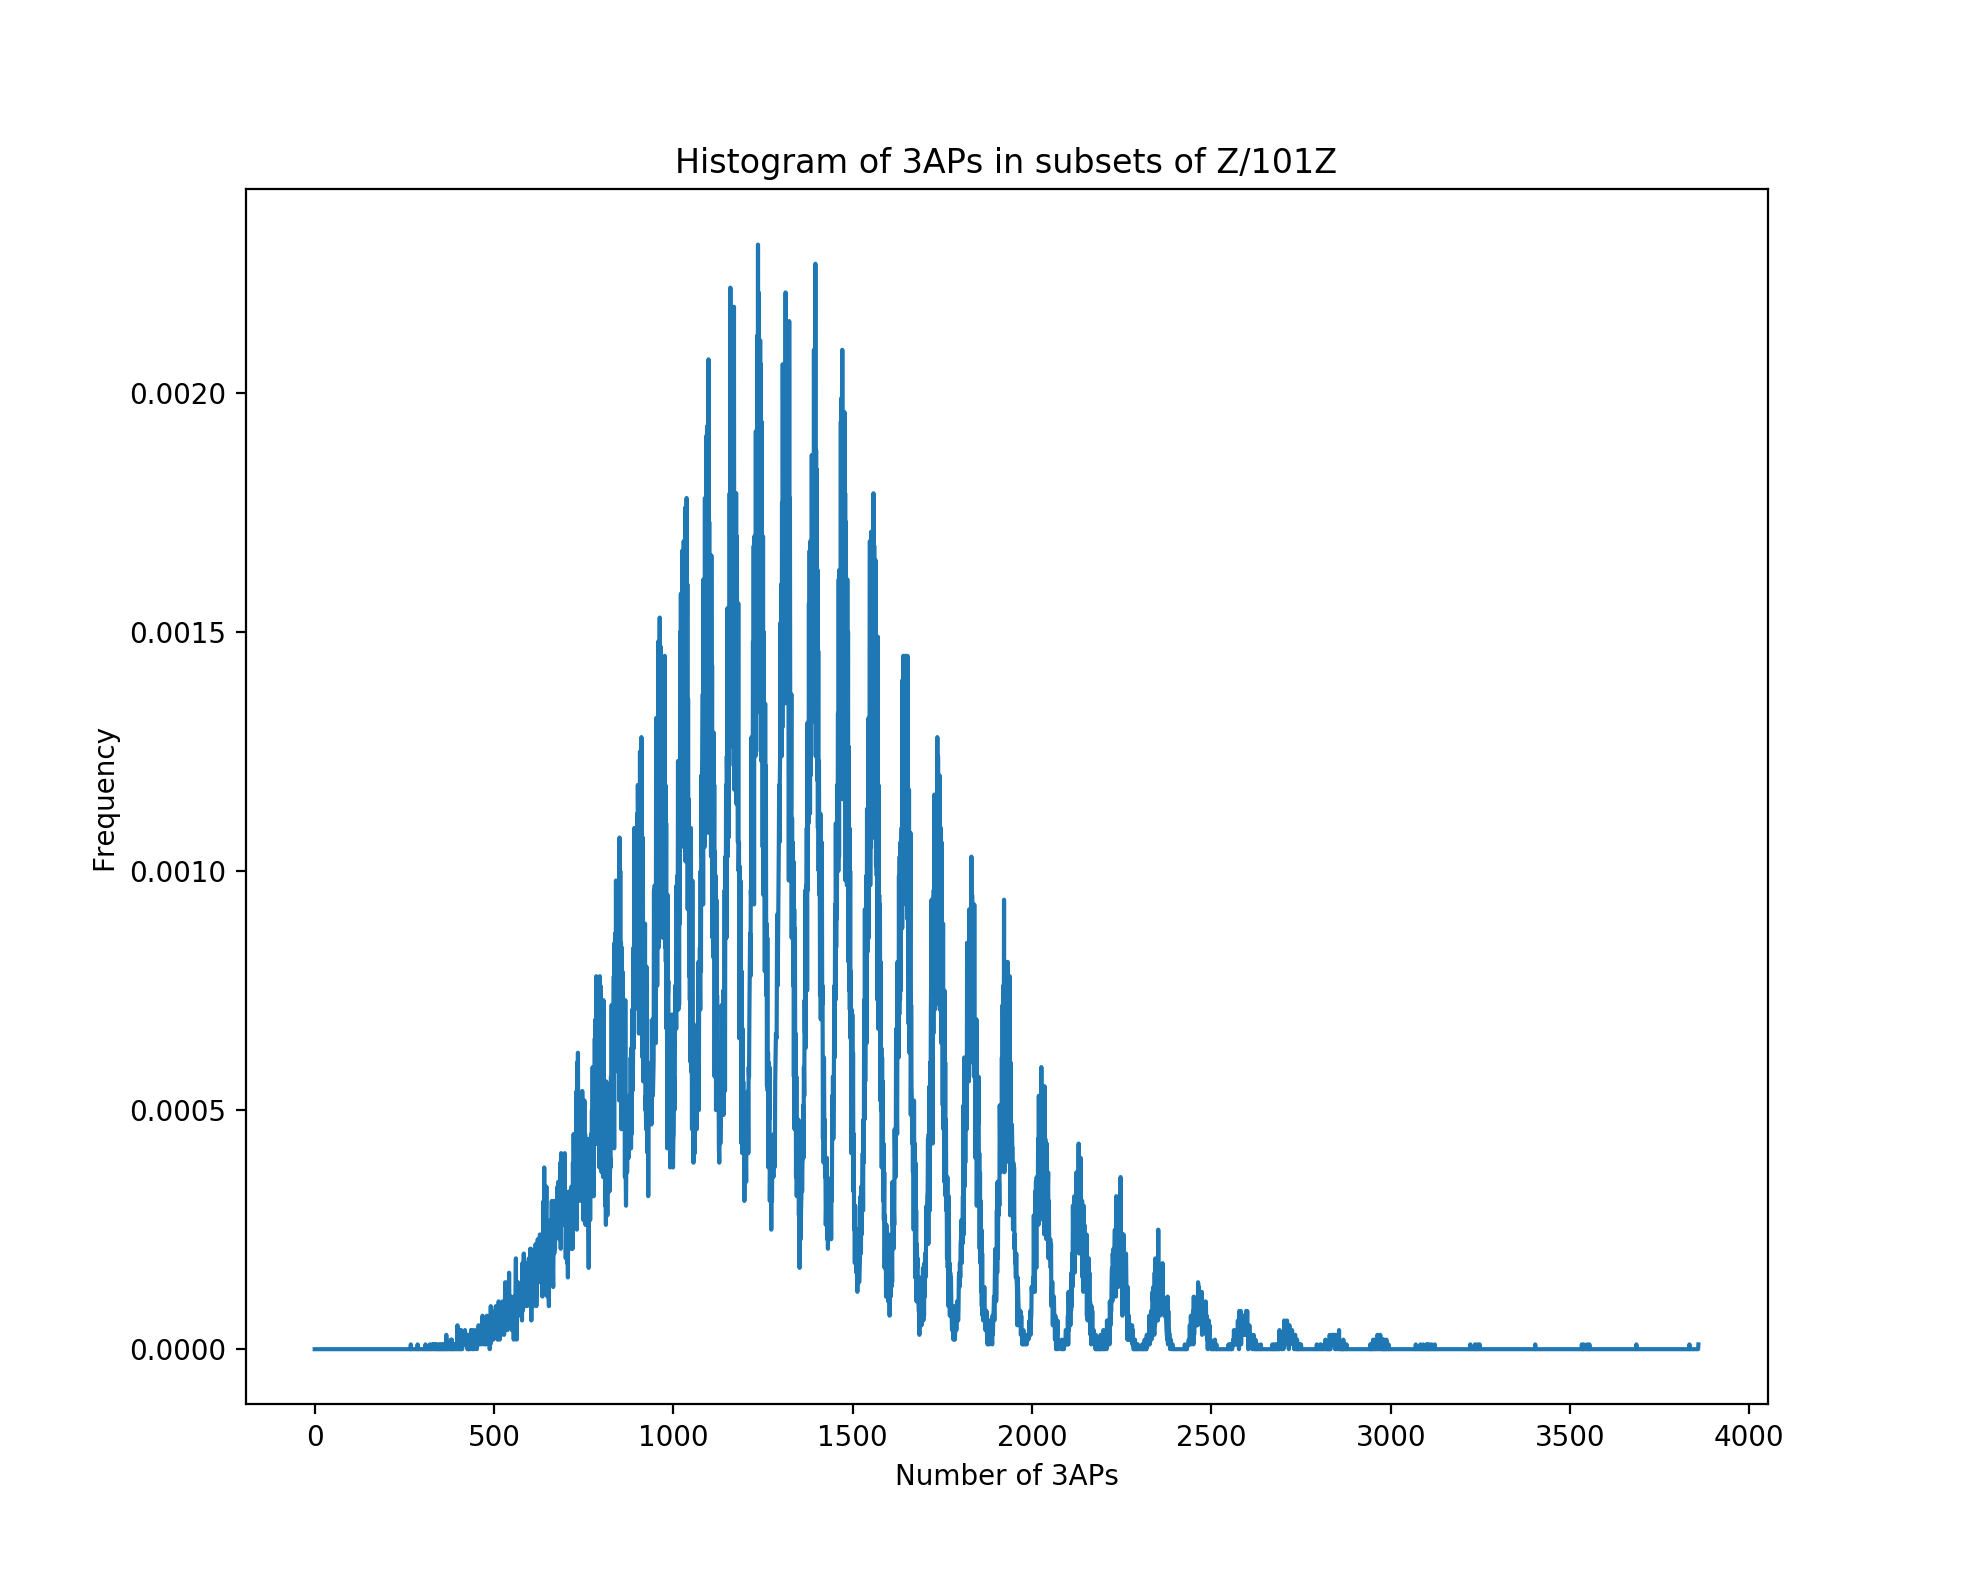
\includegraphics[scale=0.5]{3ap-hist}
    \caption{Histogram of the number of 3-term arithmetic progressions in 100,000 random subsets of $\Z / 101\Z$.}
    \label{fig:3ap}
\end{figure}

As figure \ref{fig:3ap} demonstrates, the number of arithmetic progressions in a random subset of $\Z / n \Z$ does not follow the Gaussian distribution pointwise. However, after some inspection, one might notice that the oscillations in the histogram are spaced out almost evenly. Furthermore, the oscillations themselves appear fairly Gaussian, almost as if the entire distribution is the sum of several spaced out Gaussians. Given that the spacings appear to be $O(n)$ and the entire distribution ranges from 0 to $\binom{n}{2} = O(n^2)$, we would expect there to be $O(n)$ of these smaller Gaussians. It is thus reasonable to conclude that the number of 3-term arithmetic progressions in a random subset of $\Z / n\Z$ depends on some other random variable which can take $O(n)$ values.

\begin{figure}[h]
	\centering
    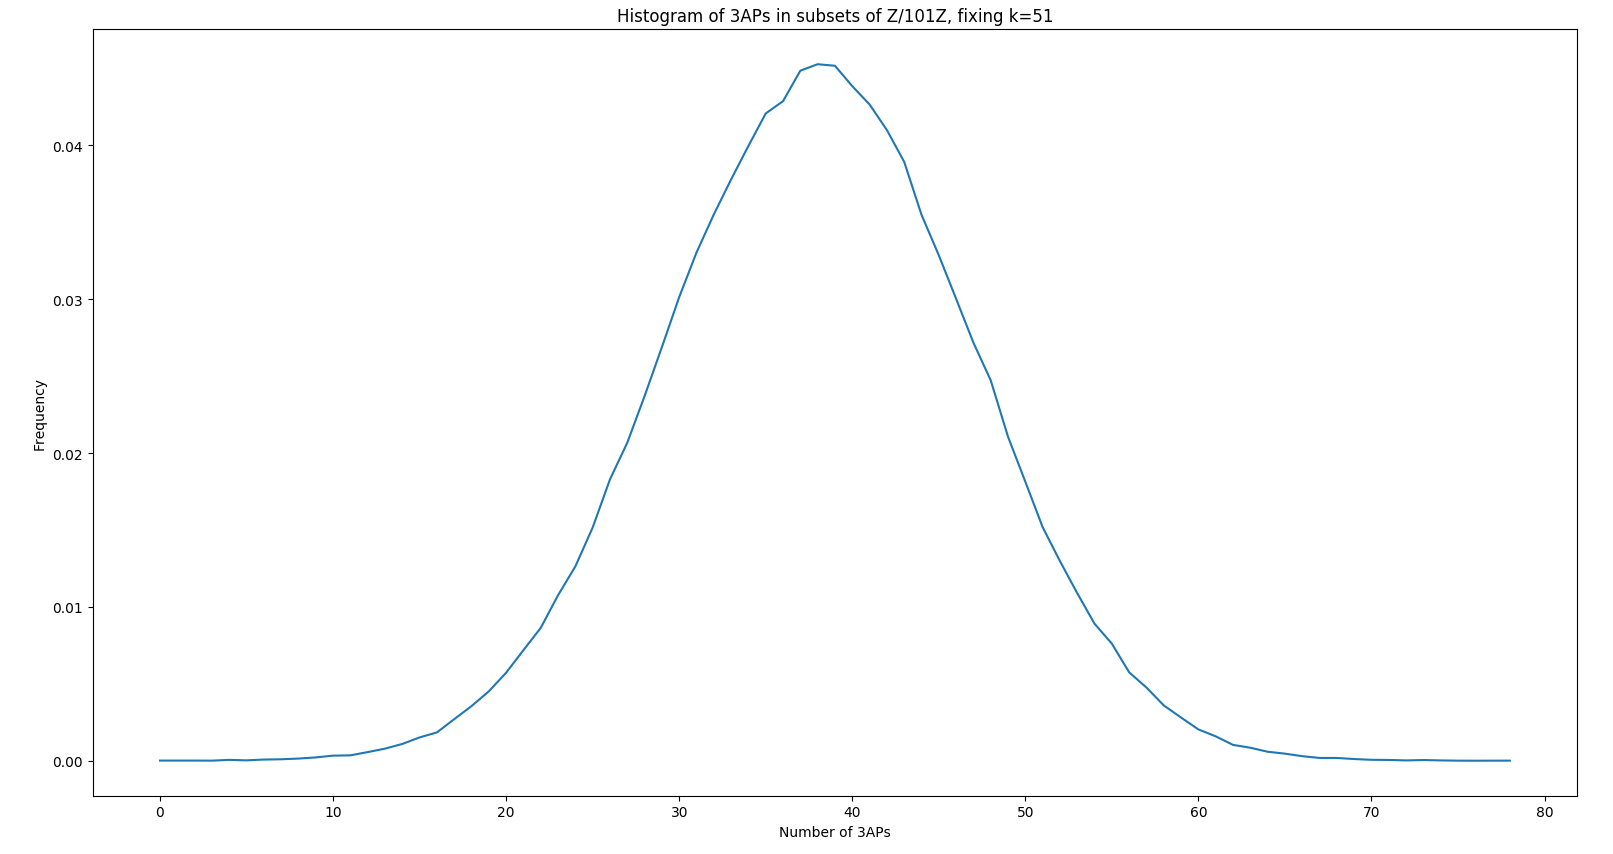
\includegraphics[scale=0.25]{3ap-fixed-k}
    \caption{Histogram of the number of 3-term arithmetic progressions in 200,000 random subsets of size 51 of $\Z / 101\Z$}
    \label{fig:3ap-k}
\end{figure}

A good guess for this other random variable is the size of a random set of $\Z / n\Z$. From figure \ref{fig:3ap-k} we can see that the number of 3-term arithmetic progressions in a random subset of $\Z / n \Z$ with fixed size does, in fact, follow the Gaussian distribution pointwise. From now on, we call this random variable $A_{n, k}$, where $k$ is the fixed size of the random subset of $\Z / n\Z$.

Therefore, we conjecture that the distance between these smaller distributions, $\E[A_{n,k+1}]-\E[A_{n,k}]$, is sufficiently smaller than the standard deviation of the distributions themselves, $\sqrt{Var(A_{n, k})}$. In other words, there is a non-trivial interval between $\E[A_{n, k}]$ and $\E[A_{n, k+1}]$ where for all x in the interval, $P(A_{n, k}=x)$ and $P(A_{n, k+1} = x)$ are both very small. In particular, we suspect that those two probabilities are significantly smaller than the Gaussian approximation of $P(A_n = x)$ would suggest.

This train of thought will be made more precise in sections 6 and 7.

\subsubsection{Continuous sets}

The first thing that should come to one's mind after observing that $A_n$ does not have an LLT due to the dependence on the size of the random set, is whether $A_n$ would have an LLT if the size of the set was made continuous. That is to say, the variable $x_i$ which denotes whether an element $i$ of $\Z / n\Z$ is in our random set $S$, is now a uniform random variable on [0, 1] instead of a Bernoulli random variable on \{0, 1\} with $p=\frac{1}{2}$. The number of arithmetic progressions $\bar{A}_n$ is still defined in a similar manner,

$$ \bar{A}_n = \frac{1}{2}\sum_{i = 1}^{n} {\sum_{j = 1}^{n-1} {x_i x_{i+j} x_{i+2j}}} $$

\begin{figure}[h]
	\centering
    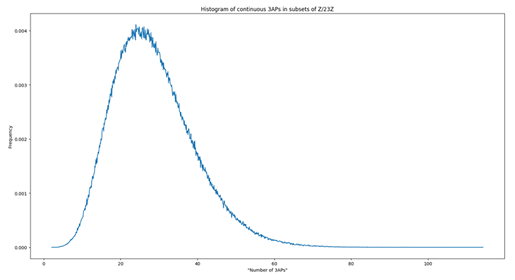
\includegraphics[scale=0.75]{3ap-cont}
    \caption{Number of 3-term "arithmetic progressions" in 1,000,000 random "continuous sets" of $\Z / 23\Z$}
    \label{fig:3ap-cont}
\end{figure}

We simulated this to see if it possibly followed the Gaussian distribution pointwise. From figure \ref{fig:3ap-cont}, we conclude that it is very likely that there is an LLT for $\bar{A}_n$. However, we have not pursued a proof of this.

\section{Attempts to get CLT or LLT for $A_{n,k}$}

\subsection*{Attempt to get CLT for $A_{n,k}$ using Stein's Method} 

In order to prove a CLT for $A_{n,k}$, we use the method of exchangeable pairs. Let $A_{n,k}$ be the number of 3-term arithmetic progressions given the subset size = $k$, and $W$ be $A_{n,k}$ standardized. We want to show that $W$ converges to a normal distribution. 
We construct $W'$ as follows. We have a random subset $S \subseteq \F_n$ with size $k$. Randomly choose two elements $I,J \in \F_n$, swap their status regarding their inclusion in $S$, and call the new subset $S'$ (i.e. if $I \in S$ and $J \not \in S$, then $I \not \in S'$ and $J \in S'$). Now define $A$ to be the number of arithmetic progressions in $S$ and define $W$ to be standardized $A$, namely $\frac{A-\mu_{n,k}}{\sigma_{n,k}}$. Similarly, define $A'$ to be the number of arithmetic progressions in $S'$ and define $W'$ to be $\frac{A'-\mu_{n,k}}{\sigma_{n,k}}$.

\remark $W$ and $W'$ are an exchangeable pair, each with mean 0 and variance 1. 

Let $\Lambda$ be a 3-term arithmtic progression  in $\F_n$. Define $1_{\Lambda \subseteq S} = 
\begin{cases} 
      1 & \Lambda \subseteq S \\
      0 & \text{else}
\end{cases}$ \\
Then $A = \sum_{\Lambda \subseteq \F_n} 1_{\Lambda \subseteq S}$. \\
Also note that $\mu_{n,k} = \E[\sum_{\Lambda \subseteq \F_n} 1_{\Lambda \subseteq S}] = \sum_{\Lambda \subseteq \F_n} P(\Lambda \in S) = \binom{n}{2}\frac{\binom{k}{3}}{\binom{n}{3}}$. \\

We first must show that $\E[W'-W\ |\ W] = -\lambda W$ for some $\lambda \in (0,1)$. 

\begin{lem}
$\lambda = \frac{3(n-k)}{\binom{n}{2}}$
\end{lem}
\begin{proof}

We have 
\[\E[A'\ |\ A] = \sum_{\Lambda \subseteq \F_n} \E[1_{\Lambda \subseteq S'}\ |\ A] = \sum_{\Lambda \subseteq \F_n} P(\Lambda \subseteq S'\ |\ A).\]

Now \[ P(\Lambda \subseteq S'\ |\ A) = P(\Lambda \subseteq S'| \Lambda \subseteq S, A)P(\Lambda \subseteq S\ |\ A) + P(\Lambda \subseteq S'\ |\ \Lambda \not \subseteq S, A)P(\Lambda \not \subseteq S\ |\ A).
\]

Note that 
\[P(\Lambda \subseteq S\ |\ A) = \frac{A}{\binom{n}{2}}\]
\[P(\Lambda \not \subseteq S\ |\ A) = 1-\frac{A}{\binom{n}{2}}\]
as there are $A$ arithmetic progressions in $S$ and $\binom{n}{2}$ arithmetic progressions total in $\F_n$.

We have \[P(\Lambda \subseteq S'\ |\ \Lambda \subseteq S, A) = 1- \frac{3(n-k)}{{{n}\choose{2}}}
\]
since the probability of $\Lambda \not \subseteq S'$ is the probability of one of its 3 elements being selected to be swapped along with one of the elements outside of $S$.

Taking this into account in our previous expression, we have
\[P(\Lambda \subseteq S'\ |\ A) = \p{1- \frac{3(n-k)}{{{n}\choose{2}}}}\p{\frac{A}{\binom{n}{2}}} + P(\Lambda \subseteq S'\ |\ \Lambda \not \subseteq S, A)\p{1-\frac{A}{\binom{n}{2}}}\]

Finally, we examine 
\begin{align*}
P(\Lambda \subseteq S'\ |\ \Lambda \not \subseteq S, A) &= \sum_{i = 0}^{3} P(\Lambda \subseteq S' \text{ and } \abs{\Lambda \cap S} = i\ |\ \Lambda \not \subseteq S \text{ and } A) \\
&= \sum_{i = 0}^{2} P(\Lambda \subseteq S'\ |\ \Lambda \not \subseteq S \text{ and } \abs{\Lambda \cap S} = i  \text{ and } A)P(\abs{\Lambda \cap S} = i\ |\ \Lambda \not \subseteq S \text{ and } A) \\
&= P(\Lambda \subseteq S'\ |\ \abs{\Lambda \cap S} = 2, \text{ and } A)P(\abs{\Lambda \cap S} = 2\ |\ \Lambda \not \subseteq S\text{ and } A).
\end{align*}

We have $P(\Lambda \subseteq S'\ |\ \abs{\Lambda \cap S} = 2, \text{ and } A) = \frac{k-2}{{n\choose2}}$ since the only way for $\Lambda$ to be contained in $S'$ if $\abs{\Lambda \cap S} = 2$ is if the one element of $\Lambda$ that is not in $S$ is chosen, along with one other element of $S \backslash \Lambda$.

Substituting this in, we get

\[P(\Lambda \subseteq S'\ |\ \Lambda \not \subseteq S, A) = \p{\frac{k-2}{{n\choose2}}}P(\abs{\Lambda \cap S} = 2\ |\ \Lambda \not \subseteq S\text{ and } A)\]

\begin{align*}
P(\abs{\Lambda \cap S} = 2\ |\ \Lambda \not \subseteq S\text{ and } A) 
&= 3P(\Lambda_1 \in S, \Lambda_2 \in S, \Lambda_3 \notin S\ |\ \Lambda \not \subseteq S \textrm{ and } A) \\
&= 3P(\Lambda_3 \notin S\ |\ \Lambda_1 \in S, \Lambda_2 \in S, \Lambda \not \subseteq S, A) \\
&\hspace{10mm} \cdot P(\Lambda_2 \in S |\ \Lambda \not \subseteq S, \Lambda_1 \in S, A)P(\Lambda_1 \in S |\ \Lambda \not \subseteq S, A) \\
&= 3P(\Lambda_2 \in S |\ \Lambda \not \subseteq S, \Lambda_1 \in S, A)P(\Lambda_1 \in S\ |\ \Lambda \not \subseteq S, A) \\
\end{align*}

Here we have two non-trivial quantities to examine. First we see by Bayes's rule that 
\begin{align*}
P(\Lambda_1 \in S\ |\ \Lambda \not \subseteq S, A) &= \dfrac{P(\Lambda \not \subseteq S\ |\ \Lambda_1 \notin S, A)P(\Lambda_1 \not \subseteq S,A)}{P(\Lambda \not \subseteq S, A)} \\
&= \dfrac{P(\Lambda \not \subseteq S\ |\ \Lambda_1 \notin S, A)P(\Lambda_1 \notin S\ |\ A)}{P(\Lambda \not \subseteq S\ |\ A)} \\
&= \dfrac{P(\Lambda \not \subseteq S\ |\ \Lambda_1 \notin S, A)\p{\frac{k}{n}}}{1-\frac{A}{\binom{n}{2}}} \\
\end{align*}

Further, we also have by Bayes's rule
\begin{align*}
P(\Lambda_2 \in S |\ \Lambda \not \subseteq S, \Lambda_1 \in S, A) &= \dfrac{P(\Lambda \not \subseteq S\ |\ \Lambda_2 \in S, \Lambda_1 \in S, A)P(\Lambda_2 \in S, \Lambda_1 \in S, A)}{P(\Lambda \not \subseteq S, \Lambda_1 \in S, A)} \\
&= \dfrac{P(\Lambda \not \subseteq S\ |\ \Lambda_2 \in S, \Lambda_1 \in S, A)P(\Lambda_2 \in S\ |\ \Lambda_1 \in S, A)}{P(\Lambda \not \subseteq S\ |\ \Lambda_1 \in S, A)} \\
&= \dfrac{P(\Lambda_3 \notin S\ |\ \Lambda_2 \in S, \Lambda_1 \in S, A)P(\Lambda_2 \in S\ |\ \Lambda_1 \in S, A)}{P(\Lambda \not \subseteq S\ |\ \Lambda_1 \in S, A)} \\
&= \dfrac{\p{1-\frac{k-2}{n-2}}\p{\frac{k-1}{n-1}}}{P(\Lambda \not \subseteq S\ |\ \Lambda_1 \in S, A)} \\
\end{align*}

So,
\begin{align*}
P(\abs{\Lambda \cap S} = 2\ |\ \Lambda \not \subseteq S\text{ and } A) &= 3\p{\dfrac{P(\Lambda \not \subseteq S\ |\ \Lambda_1 \notin S, A)\p{\frac{k}{n}}}{1-\frac{A}{\binom{n}{2}}}}\p{\dfrac{\p{1-\frac{k-2}{n-2}}\p{\frac{k-1}{n-1}}}{P(\Lambda \not \subseteq S\ |\ \Lambda_1 \in S, A)}} \\
&= 3\ \frac{\p{1-\frac{k-2}{n-2}}\p{\frac{k-1}{n-1}}\p{\frac{k}{n}}}{1-\frac{A}{{n\choose2}}}
\end{align*}

Thus, we have 
\[P(\Lambda \subseteq S'\ |\ \Lambda \not \subseteq S, A) = 3 \p{\frac{\p{1-\frac{k-2}{n-2}}\p{\frac{k-1}{n-1}}\p{\frac{k}{n}}}{\p{1-\frac{A}{{n\choose2}}}}}\p{\frac{k-2}{{n\choose2}}} = 3\p{\frac{M}{{n\choose2} - A}}\], where $M = (n-k)\frac{{k\choose3}}{{n\choose3}}$. Hence,
\[P(\Lambda \subseteq S'\ |\ A) = \p{1 - \frac{3(n-k)}{{n\choose2}}}\p{\frac{A}{{n\choose2}}} + 3\p{\frac{M}{{n\choose2}}}
\],
and so
\begin{align*}
\E[A' - A\ |\ A] &= -A + \sum_{\Lambda \subseteq \F_n} P(\Lambda \subseteq S'\ |\ A)= -A + \p{1 - \frac{3(n-k)}{{n\choose2}}}\p{A} + 3\p{M} \\
&= -\p{\frac{3(n - k)}{{n\choose2}}}(A) + 3(n-k)\frac{{k\choose3}}{{n\choose3}} \\
&= -\frac{3(n-k)}{{n\choose2}}\p{A-\binom{n}{2}\frac{\binom{k}{3}}{\binom{n}{3}}} \\
&= -\frac{3(n-k)}{{n\choose2}}(A-\mu).
\end{align*}
Thus, 
$\E[A'-A |A] = -\lambda(A-\mu)$, where $\lambda = \frac{3(n-k)}{{n\choose2}}$. 
Hence, $\E[W'-W|W] = \E[\frac{A'-\mu}{\sigma} - \frac{A-\mu}{\sigma}] = \frac{1}{\sigma}\E[A'-A] = -\lambda\p{\frac{A-\mu}{\sigma}} = -\lambda W$.


\end{proof}

Thus, using the method of exchangeable pairs, we can bound the Wasserstein distance $Wass(W, Z)$, where $Z$ is a standard Gaussian random variable:
\[Wass(W,Z) \leq \sqrt{\p{\frac{2}{\pi}}\textrm{Var}(\E[\frac{1}{2\lambda}(W'-W)^2 | W])} + \frac{1}{3\lambda}\E[\abs{W'-W}^2]\].
Now $\E[\frac{1}{2\lambda}(W'-W)^2 | W] = \E[\frac{{n\choose2}}{6(n-k)}(W'-W)^2 | W] = \frac{{n\choose2}}{6(n-k)}(\E[(W')^2|W]-2\E[WW'|W]+W^2)$.


\subsection{Attempt to get LLT for $A_{n,k}$}
The main issue that we run into when trying to apply the same technique used to show LLTs for $T_n$ and $D_n$ to $A_{n,k}$ is that we cannot find an event to condition on such that $A_{n,k}$ will depend 



\section{General Framework for no LLT for other R.V.'s}
We want to develop an overarching framework for what properties a random variable $X_n$ must have so that it follows a CLT but not an LLT. Let $X_n$ be conditioned on some event with values denoted by $k$. 

Let gap $g = (\mu_{k+1}-\mu_k) \sim f(n,k) = \Omega(\sigma_{n,k}\sigma_n^{\epsilon})$ for some $\epsilon >0$.
We proceed to show the following short proposition, which establishes a condition for which $X_n$ does not satisfy a LLT:
\begin{prop}
If we pick $x$ such that $\abs{x - \mu_n} = \Omega(f(n,k)) = \omega(\sigma_{n,k}) \ \forall k$, then $\abs{P(X_n = x) - \mathcal{N}_n(x)} = \Omega(\frac{1}{\sigma_n})$.
\end{prop}
\begin{proof} We have
\[P(X_n = x) = \sum_{k = 1}^j P(Y_k)P(X_n = x | Y)k) \leq \sum_{k = 1}^j P(\abs{X_n-\mu_k} \geq \abs{x-\mu_k}) P(Y_k) \leq \sum_{k=1}^j \p{\frac{\sigma_{n,k}}{\abs{x-\mu_k}}}^2 P(Y_k) \] by Chebyshev's Inequality.
Now $\p{\frac{\sigma_{n,k}}{\abs{x-\mu_k}}} = o(\frac{1}{\sigma_n^{\epsilon}})$, so $\p{\frac{\sigma_{n,k}}{\abs{x-\mu_k}}}^2 = o(\frac{1}{\sigma_n})$. Now $\mathcal{N}_n(x) = \frac{1}{\sqrt{2\pi}\sigma_n} e^{-\p{\frac{x-\mu_n}{\sigma_n}}^2/2} = O(\frac{1}{\sigma_n})$. Hence, $\abs{P(X_n = x) - \mathcal{N}_n(x)} = \Omega(\frac{1}{\sigma_n})$ and thus $X_n$ does not follow a LLT. 

\end{proof}



\section{Attempt to prove no LLT for $A_n$}

To show that there is no LLT for $A_n$, our strategy is to choose a point $x$ in the middle between two $A_{n,k}$ distributions and showing that $\abs{P(A_n = x) - \mathcal{N}_n(x)} = \Omega(\frac{1}{\sigma_n})$, where $\mathcal{N}_n(x) = \frac{1}{\sqrt{2\pi}\sigma_n} e^{((x-\mu_n)/\sigma_n)^{2}/2}$. 

Set $p = \frac{1}{2}$, and let $x \geq \mu_{n,k} \ \forall k \leq j \text{ and } x \leq \mu_{n,k} \ \forall k>j$. Then we have
\begin{align*}
P(A_n = x) &= \sum_{k = 0}^n P(A_n = x |\ |S| = k)P(|S| = k)\\
&= \sum_{k = 0}^n P(A_{n,k} = x) \cdot \frac{{n\choose k}}{2^n} \\
&\leq \sum_{k = 0}^j P(A_{n,k} \geq x) \cdot \frac{{n\choose k}}{2^n} + \sum_{k = j+1}^n P(A_{n,k} \leq x) \cdot \frac{{n\choose k}}{2^n}
\end{align*}

Now we must sufficiently bound the tails of $A_{n,k}$. We know that $\mu_{A_n} = \frac{1}{8}{n\choose 2} \sigma_{A_n}^2 = \Theta(n^3), \mu_{n,k} = \frac{3}{n-2} {k\choose 3}, \text{ and } \sigma_{A_{n,k}}^2 = \frac{k^3(n-k)^3}{2n^4}$, but we do not know anything about the shape of the distribution of $A_{n,k}$. 
Thus, we first try using Chebyshev's Inequality...

% TODO: showing a high point is too high instead of showing a low point is too low

\bibliographystyle{plain}
\begin{thebibliography}{0}
		\bibitem{GilmerKopparty14}
			Justin Gilmer and Swastik Kopparty.
			A local central limit theorem for the number of triangles in a random graph.
			\emph{ArXiv e-prints},
			November 2014.
		\bibitem{Fulman97}
			Jason Fulman.
			Stein's Method and Non-Reversible Markov Chains.
			\emph{ArXiv e-prints},
			December 1997.
        \bibitem{Chatterjee07}
			Sourav Chatterjee.
			Lecture Notes in Stein's method and applications.
			August 2007.
			Retrieved August 14, 2018 from https://statweb.stanford.edu/\textasciitilde{}souravc/Lecture1.pdf.
\end{thebibliography}


\end{document}
